\documentclass{standalone}
\usepackage{graphicx}	
\usepackage{amssymb, amsmath}
\usepackage{color}

\usepackage{tikz}
\usetikzlibrary{intersections, backgrounds}

\definecolor{light}{RGB}{220, 188, 188}
\definecolor{mid}{RGB}{185, 124, 124}
\definecolor{dark}{RGB}{143, 39, 39}
\definecolor{highlight}{RGB}{180, 31, 180}
\definecolor{gray10}{gray}{0.1}
\definecolor{gray20}{gray}{0.2}
\definecolor{gray30}{gray}{0.3}
\definecolor{gray40}{gray}{0.4}
\definecolor{gray60}{gray}{0.6}
\definecolor{gray70}{gray}{0.7}
\definecolor{gray80}{gray}{0.8}
\definecolor{gray90}{gray}{0.9}
\definecolor{gray95}{gray}{0.95}

\newcommand*{\offset}{0.025}

\begin{document}

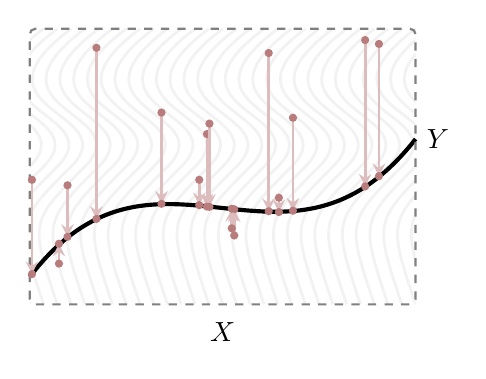
\begin{tikzpicture}[scale=0.35, thick]
  \begin{scope}
    \clip (5, 0) rectangle +(14, 10);
    \foreach \i in {2.5, 3, ..., 21.5} {
      \draw [color=gray95, line width=1] (\i, 0) .. controls +(-1, 3) .. +(1, 5) .. 
                                         controls +(2, 2) and +(-4, -3) .. +(1, 10);
  }  
  \end{scope}
  
  \node at (12, -1) { $X$ };
    
  \draw [line width=1.5] (5, 1) .. controls (9.6, 7) and (14.3, 0) .. (19, 6)
  node[right] { $Y$ };
  
  \draw [rounded corners=2pt, color=gray, dashed] (5, 0) rectangle +(14, 10);
  
  \draw [->, >=stealth, line width=1, color=light] (14.55, 6.77) -- (14.55, 3.4);
  \fill [fill=mid] (14.55, 6.77) circle (0.15);
  \fill [fill=mid] (14.55, 3.4) circle (0.15);
  
  \draw [->, >=stealth, line width=1, color=light] (13.67, 9.12) -- (13.67, 3.38);
  \fill [fill=mid] (13.67, 9.12) circle (0.15);
  \fill [fill=mid] (13.67, 3.38) circle (0.15);
  
  \draw [->, >=stealth, line width=1, color=light] (12.42, 2.50) -- (12.42, 3.45);
  \fill [fill=mid] (12.42, 2.50) circle (0.15);
  \fill [fill=mid] (12.42, 3.45) circle (0.15);
  
  \draw [->, >=stealth, line width=1, color=light] (17.67, 9.45) -- (17.67, 4.65);
  \fill [fill=mid] (17.67, 9.45) circle (0.15);
  \fill [fill=mid] (17.67, 4.65) circle (0.15);
 
  \draw [->, >=stealth, line width=1, color=light] (11.15, 4.52) -- (11.15, 3.6);
  \fill [fill=mid] (11.15, 4.52) circle (0.15);
  \fill [fill=mid] (11.15, 3.6) circle (0.15);
  
  \draw [->, >=stealth, line width=1, color=light] (5.08, 4.52) -- (5.08, 1.1);
  \fill [fill=mid] (5.08, 4.52) circle (0.15);
  \fill [fill=mid] (5.08, 1.1) circle (0.15);
   
  \draw [->, >=stealth, line width=1, color=light] (6.06, 1.48) -- (6.06, 2.2);
  \fill [fill=mid] (6.06, 1.48) circle (0.15);
  \fill [fill=mid] (6.06, 2.2) circle (0.15);
  
  \draw [->, >=stealth, line width=1, color=light] (11.43, 6.18) -- (11.43, 3.55);
  \fill [fill=mid] (11.43, 6.18) circle (0.15);
  \fill [fill=mid] (11.43, 3.55) circle (0.15);
  
  \draw [->, >=stealth, line width=1, color=light] (14.04, 3.87) -- (14.04, 3.35);
  \fill [fill=mid] (14.04, 3.87) circle (0.15);
  \fill [fill=mid] (14.04, 3.35) circle (0.15);
  
  \draw [->, >=stealth, line width=1, color=light] (6.37, 4.32) -- (6.37, 2.45);
  \fill [fill=mid] (6.37, 4.32) circle (0.15);
  \fill [fill=mid] (6.37, 2.45) circle (0.15);
   
  \draw [->, >=stealth, line width=1, color=light] (12.33, 2.76) -- (12.33, 3.47);
  \fill [fill=mid] (12.33, 2.76) circle (0.15);
  \fill [fill=mid] (12.33, 3.47) circle (0.15);
  
  \draw [->, >=stealth, line width=1, color=light] (9.78, 6.96) -- (9.78, 3.65);
  \fill [fill=mid] (9.78, 6.96) circle (0.15);
  \fill [fill=mid] (9.78, 3.65) circle (0.15);
  
  \draw [->, >=stealth, line width=1, color=light] (11.52, 6.56) -- (11.52, 3.54);
  \fill [fill=mid] (11.52, 6.56) circle (0.15);
  \fill [fill=mid] (11.52, 3.54) circle (0.15);
  
  \draw [->, >=stealth, line width=1, color=light] (17.17, 9.59) -- (17.17, 4.28);
  \fill [fill=mid] (17.17, 9.59) circle (0.15);
  \fill [fill=mid] (17.17, 4.28) circle (0.15);
  
  \draw [->, >=stealth, line width=1, color=light] (7.42, 9.31) -- (7.42, 3.1);
  \fill [fill=mid] (7.42, 9.31) circle (0.15);
  \fill [fill=mid] (7.42, 3.1) circle (0.15);

\end{tikzpicture}

\end{document}  